\section{Spheres}
\begin{figure}[H]
\centering
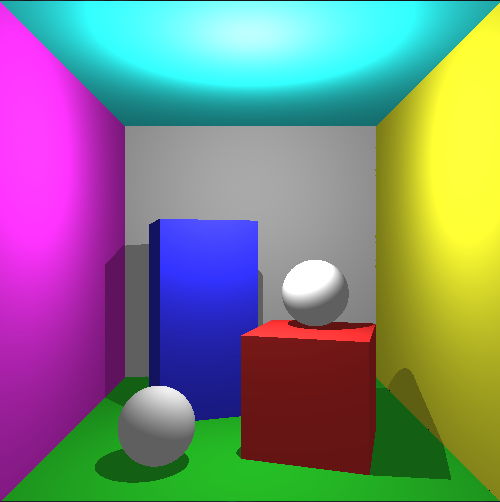
\includegraphics[width=0.4\linewidth]{img/spheres.jpg}
\caption{Spheres (930 ms)}
\end{figure}


\section{Ray-triangle intersection: optimization}
New ray/triangle intersection algorithm:
http://en.wikipedia.org/wiki/M%C3%B6ller%E2%80%93Trumbore_intersection_algorithm (3 times faster, 360ms)


\section{Specular materials}
\begin{figure}[H]
\centering
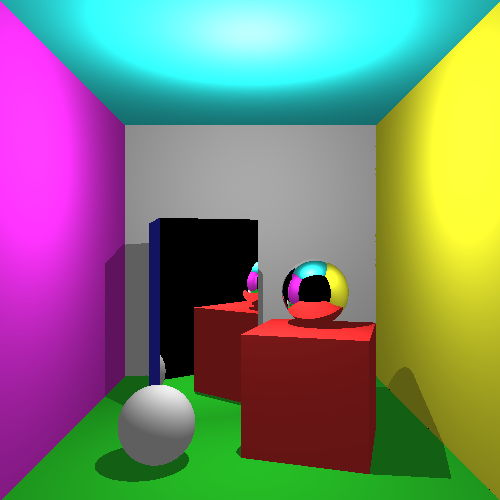
\includegraphics[width=0.4\linewidth]{img/specular.jpg}
\caption{Specular materials}
\end{figure}


\section{Glass - Refraction}
\begin{figure}[H]
\centering
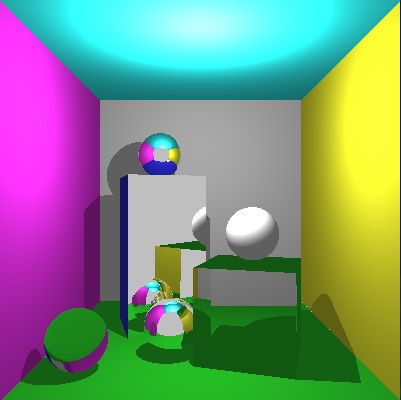
\includegraphics[width=0.4\linewidth]{img/glass_refraction.jpg}
\caption{Refraction through glass (430 ms)}
\end{figure}


\section{Anti-aliasing}
\subsection{Edges detection}


\begin{figure}[H]
\centering
\minipage[t]{0.4\textwidth}
    \centering
    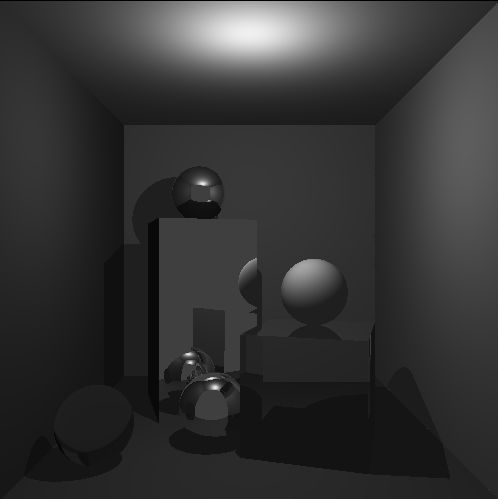
\includegraphics[width=\linewidth]{img/antialiasing/grayscale.jpg}
    \caption{Grayscale scene}
\endminipage
\minipage[t]{0.4\textwidth}
    \centering
    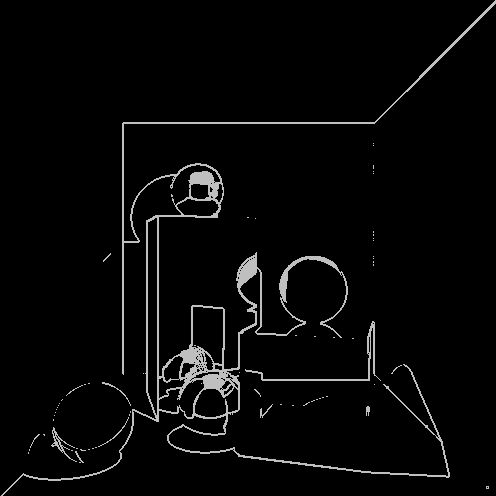
\includegraphics[width=\linewidth]{img/antialiasing/sobel.jpg}
    \caption{Edges detection (Sobel operator)}
\endminipage
\end{figure}


\subsection{Uniform}

\subsection{Stochastic sampling}

They are zoomed
\begin{figure}[H]
\minipage{0.25\textwidth}
    \centering
    
\includegraphics[width=\linewidth]{img/antialiasing/no_aa.png}
    \caption{AA disabled (430 ms)}
\endminipage\hfill
\minipage{0.25\textwidth}
    \centering
    
\includegraphics[width=\linewidth]{img/antialiasing/super8x.png}
    \caption{Uniform 8x (1200 ms)}
\endminipage\hfill
\minipage{0.25\textwidth}
    \centering
    
\includegraphics[width=\linewidth]{img/antialiasing/sto8x.png}
    \caption{Jittered 8x (1250 ms)}
\endminipage\hfill
\minipage{0.25\textwidth}
    \centering
    
\includegraphics[width=\linewidth]{img/antialiasing/sto16x.png}
    \caption{Jittered 16x (1450 ms)}
\endminipage\hfill
\end{figure}


\begin{figure}[H]
\centering
\minipage[t]{0.4\textwidth}
    \centering
    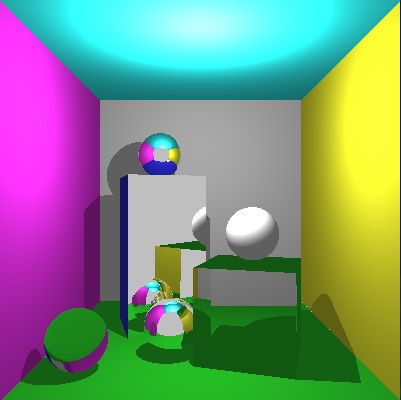
\includegraphics[width=\linewidth]{img/glass_refraction.jpg}
    \caption{Anti-aliasing disabled (430 ms)}
\endminipage
\minipage[t]{0.4\textwidth}
    \centering
    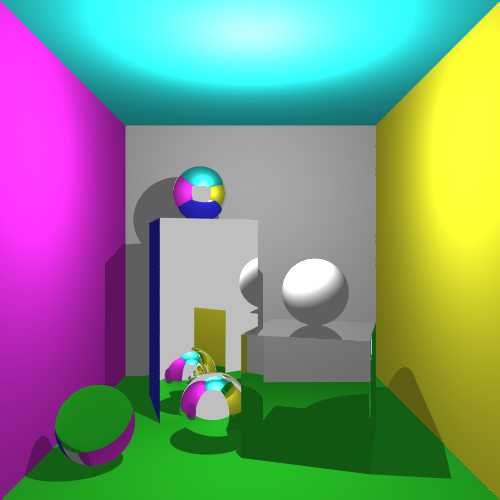
\includegraphics[width=\linewidth]{img/antialiasing/stoAA16x_full.png}
    \caption{Stochastic sampling 16x (1450 ms)}
\endminipage
\end{figure}


\section{Glass - Reflection}
20 bounces
\begin{figure}[H]
\centering
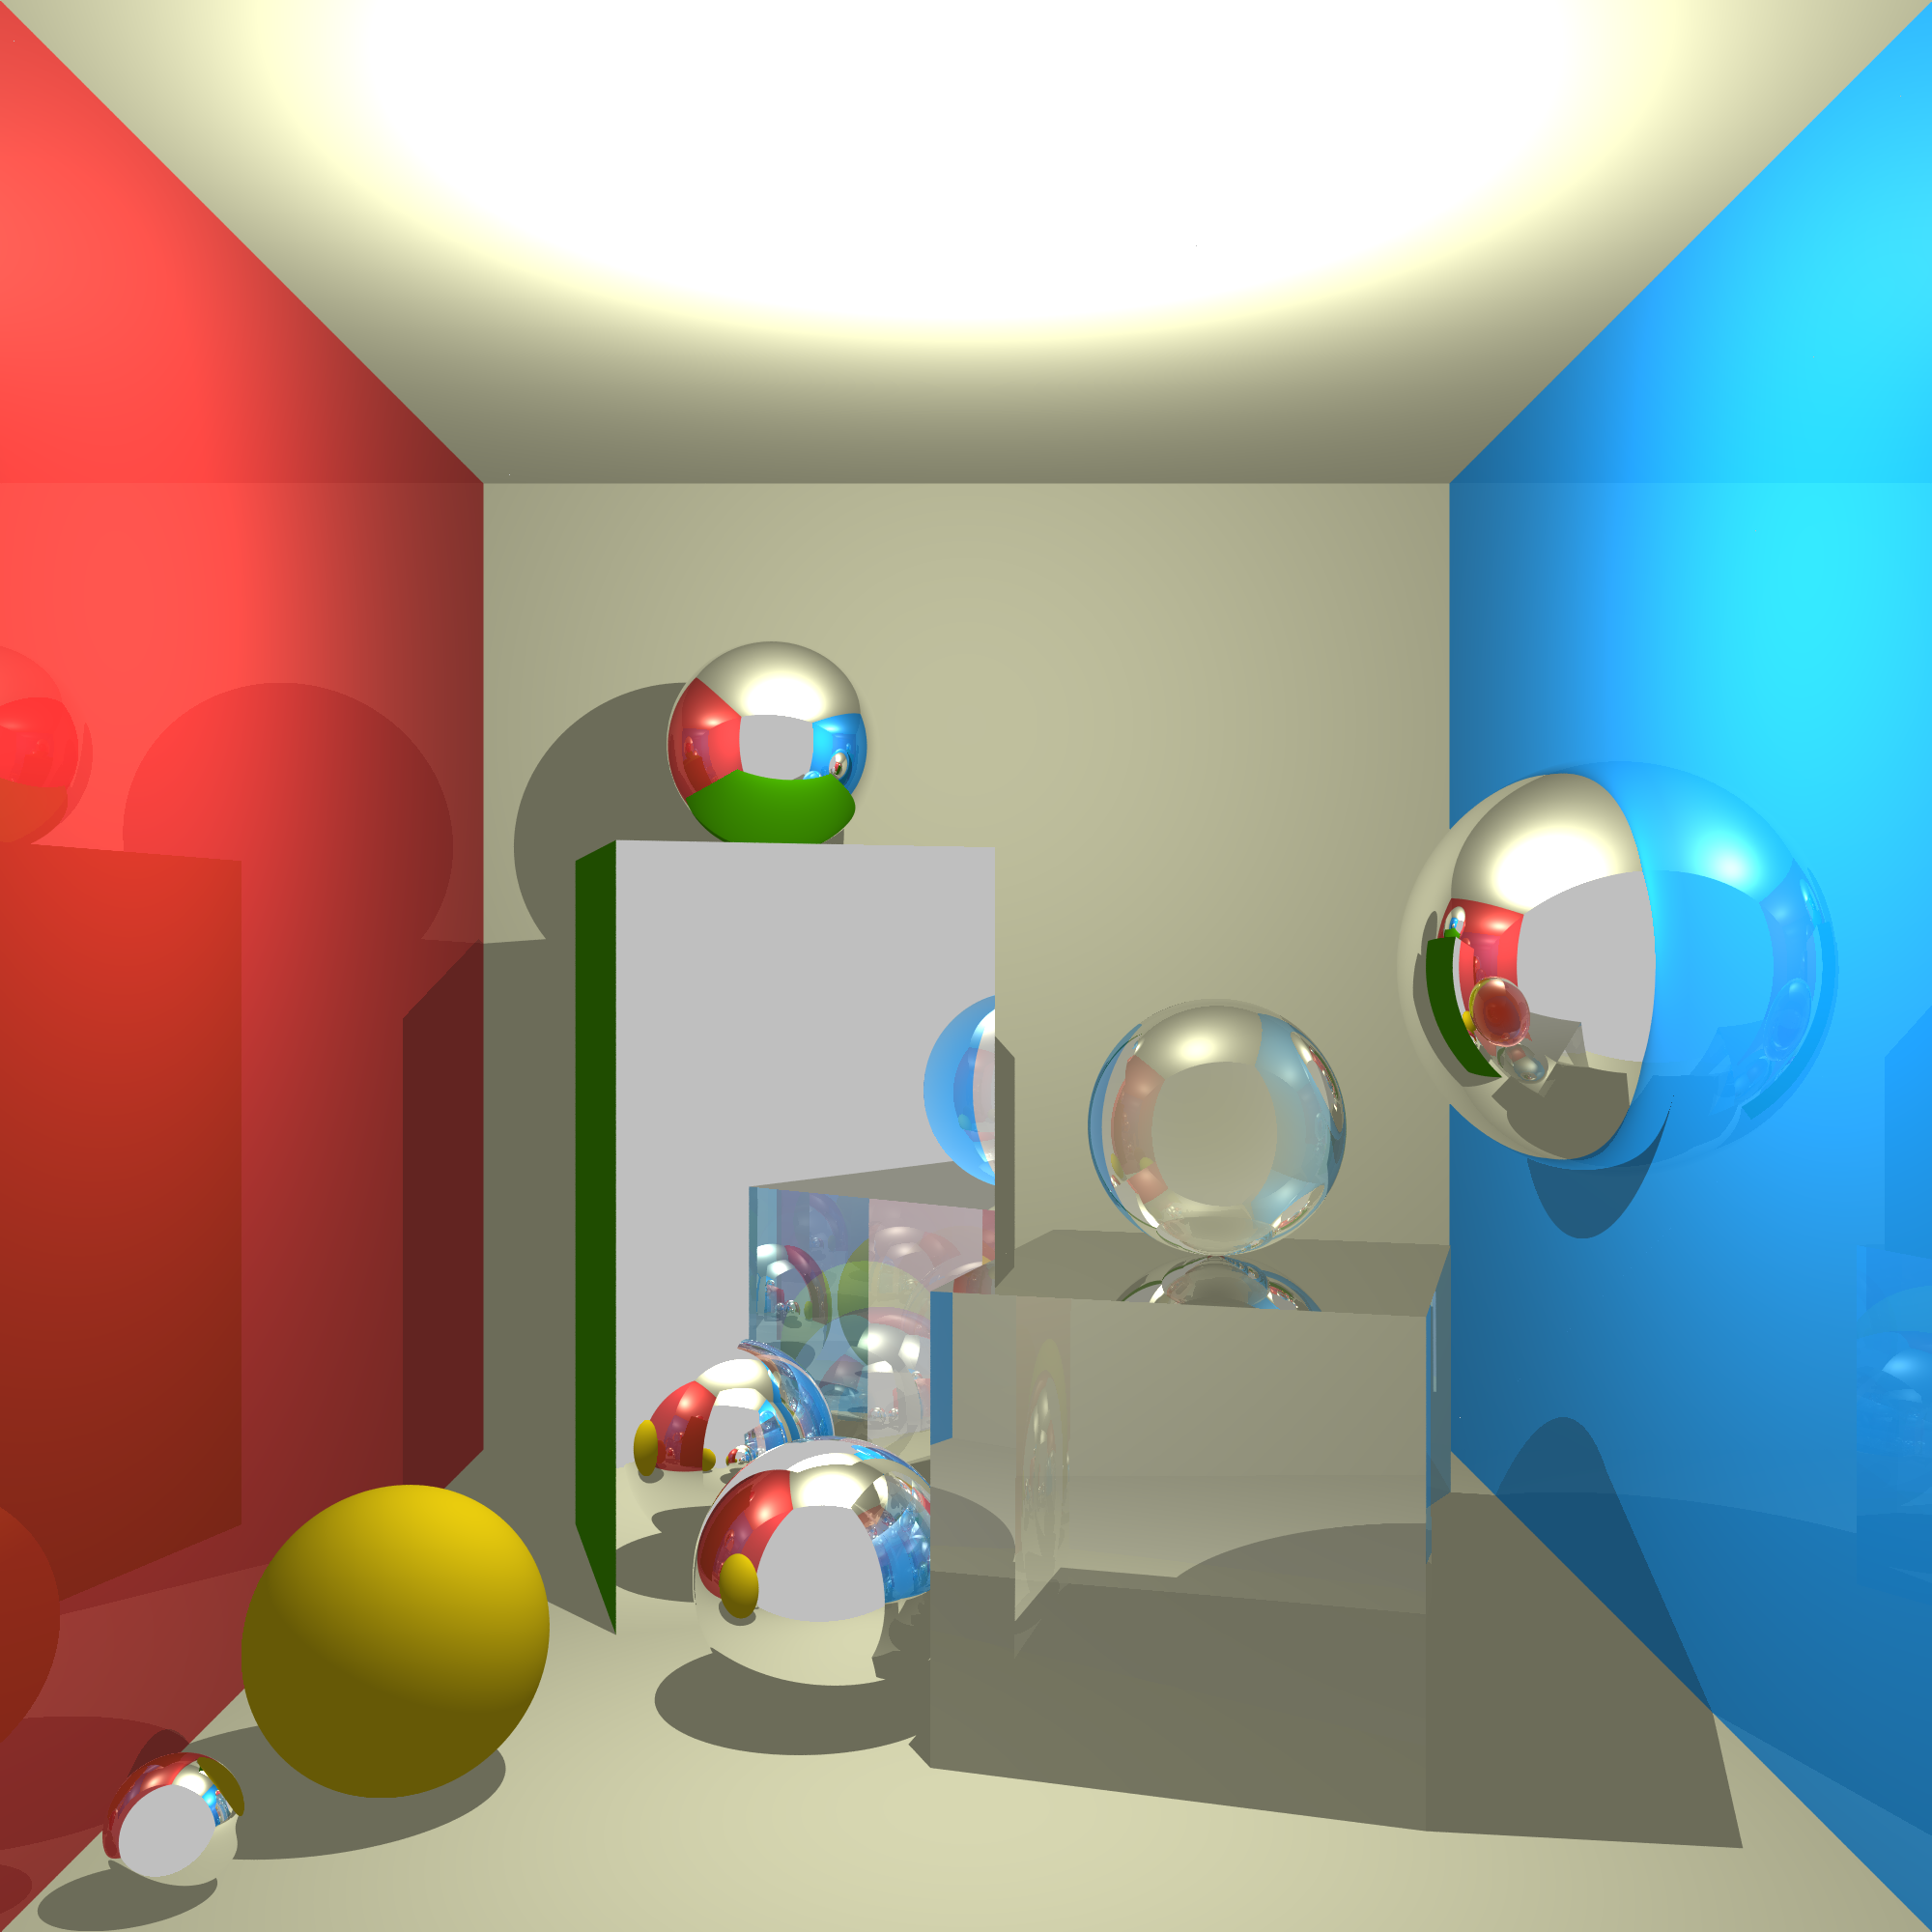
\includegraphics[width=0.4\linewidth]{img/glass_awesome.png}
\caption{Glass: refraction and reflection}
\end{figure}


\section{Soft shadows}
\subsection{Uniform light sources}
The following scenes were processed for a 500x500 resolution without anti-aliasing.
\begin{figure}[H]
\minipage{0.33\textwidth}
    \centering
    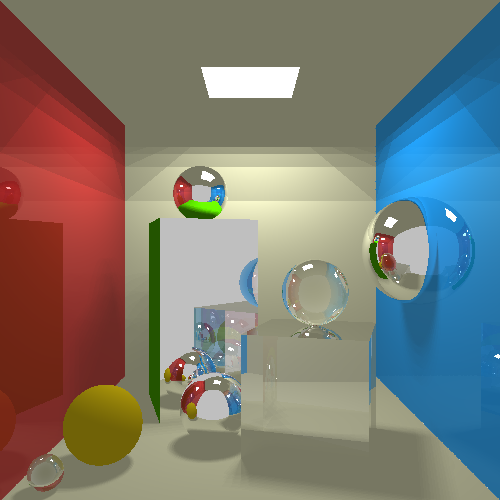
\includegraphics[width=\linewidth]{img/shadows/16.png}
    \caption{16 lights, uniform (8700 ms)}
\endminipage\hfill
\minipage{0.33\textwidth}
    \centering
    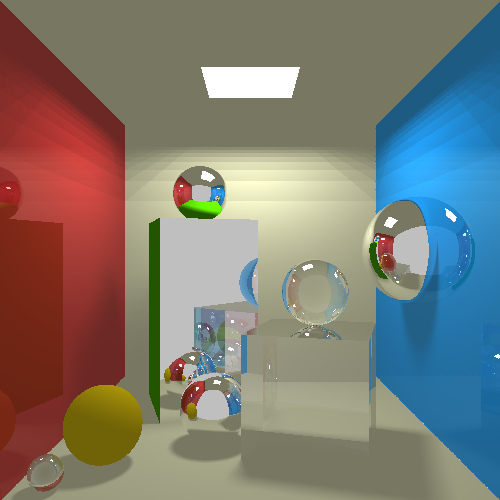
\includegraphics[width=\linewidth]{img/shadows/64.png}
    \caption{64 lights, uniform (30 600 ms)}
\endminipage\hfill
\minipage{0.33\textwidth}
    \centering
    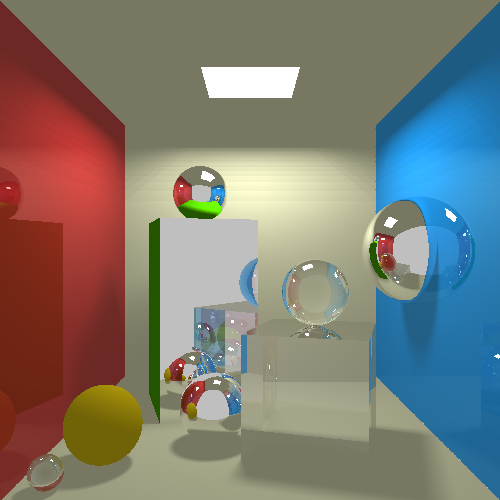
\includegraphics[width=\linewidth]{img/shadows/256.png}
    \caption{256 lights, uniform (118 500 ms)}
\endminipage\hfill
\end{figure}

\subsection{Jittered light sources}
\begin{figure}[H]
\minipage{0.33\textwidth}
    \centering
    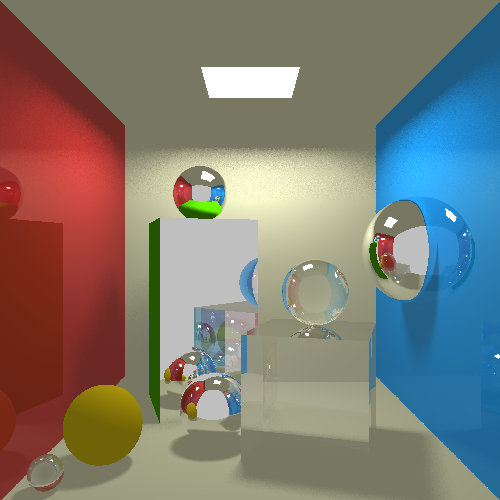
\includegraphics[width=\linewidth]{img/shadows/16_jittered.png}
    \caption{16 lights, jittered (9400 ms)}
\endminipage\hfill
\minipage{0.33\textwidth}
    \centering
    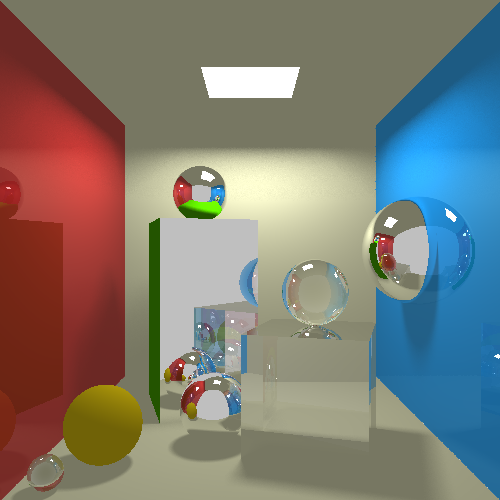
\includegraphics[width=\linewidth]{img/shadows/64_jittered.png}
    \caption{64 lights, jittered (33 600 ms)}
\endminipage\hfill
\minipage{0.33\textwidth}
    \centering
    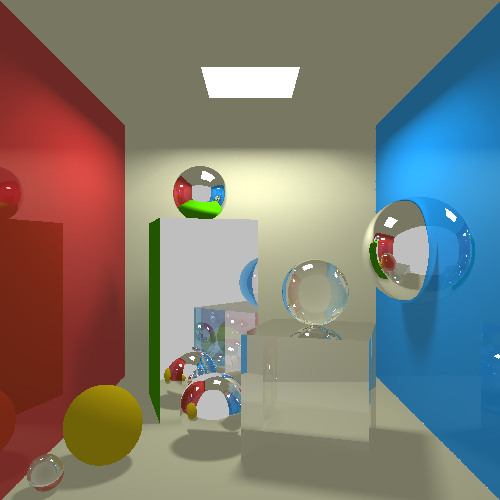
\includegraphics[width=\linewidth]{img/shadows/256_jittered.png}
    \caption{256 lights, jittered (128 600 ms)}
\endminipage\hfill
\end{figure}

%\begin{figure}[H]
%\centering
%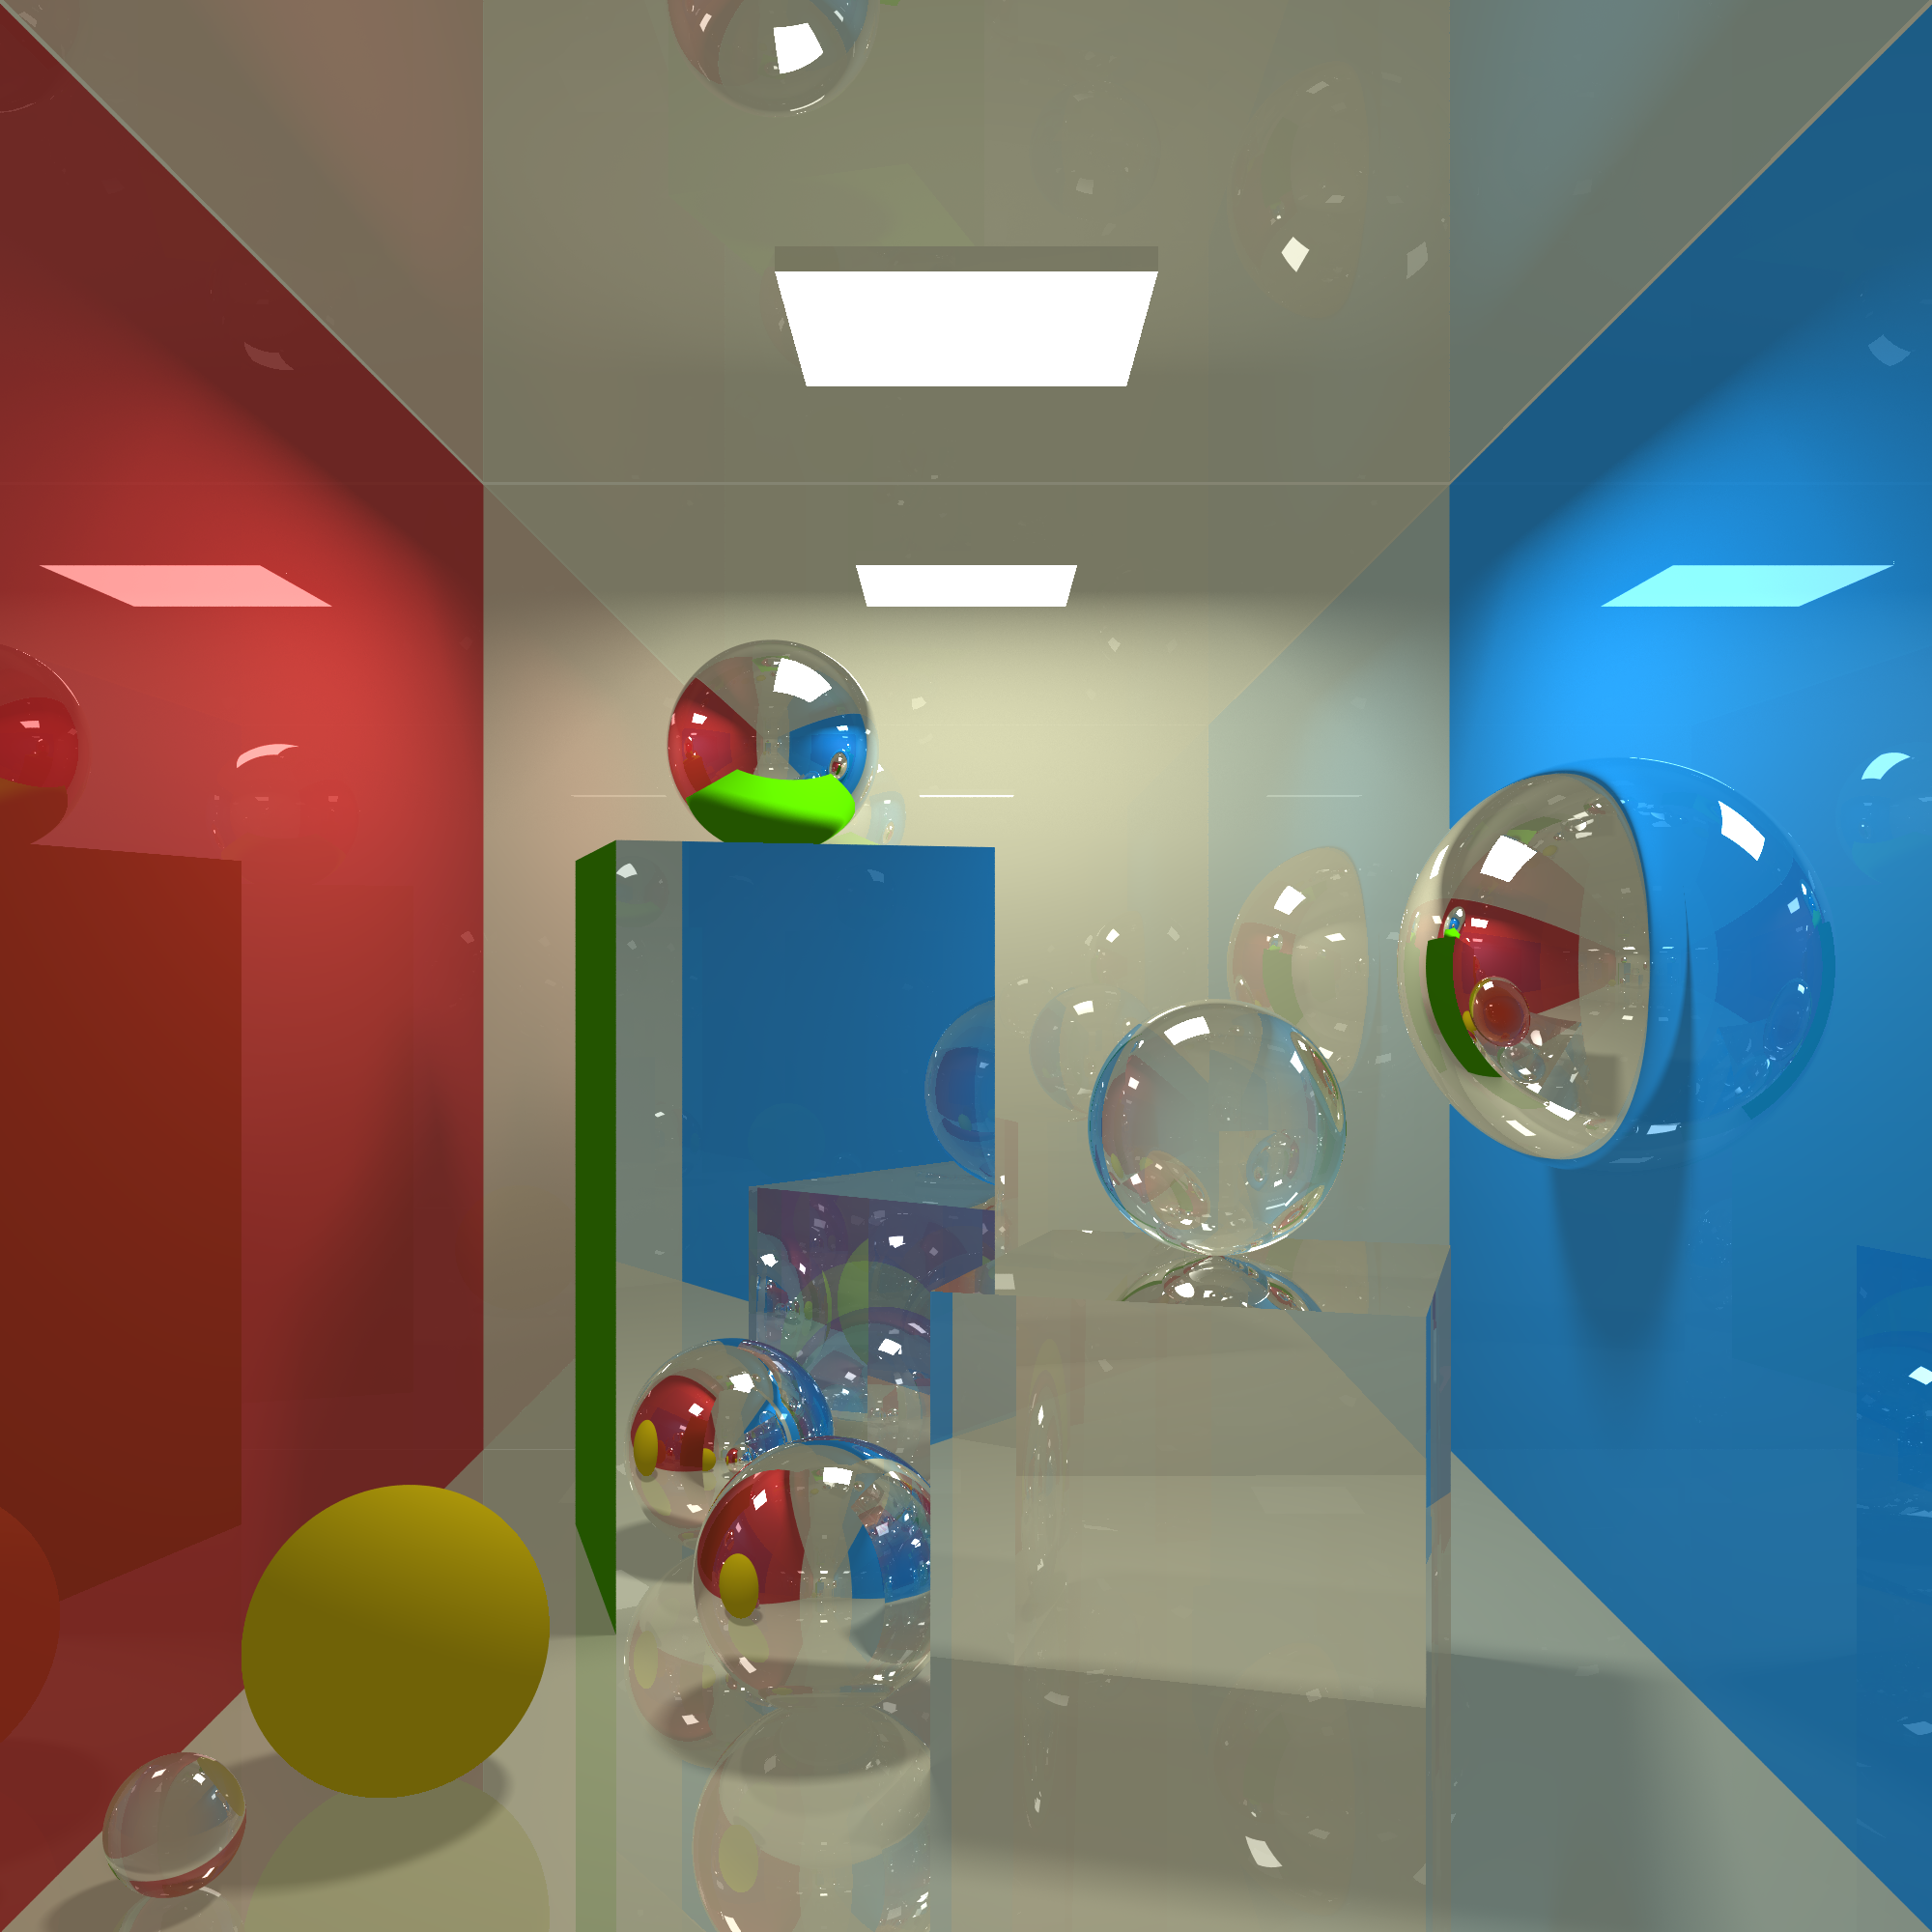
\includegraphics[width=0.4\linewidth]{img/final.png}
%\caption{Final scene}
%\end{figure}
